% Ploicy Gradient method in Evolutionary Pricing Games
\documentclass[a4paper,12pt]{article}  %% important: a4paper first

\usepackage{graphicx}
\graphicspath{{./img/}}
\usepackage[notcite,notref]{showkeys}
\pdfoutput=1
\usepackage{natbib} 
\usepackage{amsthm}
\usepackage{newpxtext,newpxmath} 
\usepackage{microtype}
\linespread{1.10}        % Palatino needs more leading (space between lines)
\usepackage{xcolor}
\usepackage{pict2e} 

\usepackage{tikz} 
\usetikzlibrary{shapes}
\usetikzlibrary{arrows.meta}

%\usepackage{smallsec}
\usepackage{graphicx}
%\usepackage[pdflatex]{hyperref}
\usepackage[hyphens]{url} 
\usepackage[colorlinks,linkcolor=purple,citecolor=blue]{hyperref}
%\usepackage{hyperref}
\urlstyle{sf}
\usepackage[format=hang,justification=justified,labelfont=bf,labelsep=quad]{caption} 
% \input macros-drawtree
\oddsidemargin=.46cm    % A4
\textwidth=15cm
\textheight=23.3cm
\topmargin=-1.3cm
\clubpenalty=10000
\widowpenalty=10000
\predisplaypenalty=1350
\sfcode`E=1000  % normal spacing if E followed by period, as in "EFCE."
\sfcode`P=1000  % normal spacing if P followed by period, as in "NP." 
\newdimen\einr
\einr1.7em
\newdimen\eeinr 
\eeinr 1.7\einr
\def\aabs#1{\par\hangafter=1\hangindent=\eeinr
	\noindent\hbox to\eeinr{\strut\hskip\einr#1\hfill}\ignorespaces}
\def\rmitem#1{\par\hangafter=1\hangindent=\einr
	\noindent\hbox to\einr{\ignorespaces#1\hfill}\ignorespaces} 
\newcommand\bullitem{\rmitem{\raise.17ex\hbox{\kern7pt\scriptsize$\bullet$}}} 
\def\subbull{\vskip-.8\parskip\aabs{\raise.2ex\hbox{\footnotesize$\circ$}}}
\let\sfield\mathcal
\newtheorem{theorem}{Theorem}
\newtheorem{corollary}[theorem]{Corollary}
\newtheorem{example}[theorem]{Example}
\newtheorem{lemma}[theorem]{Lemma}
\newtheorem{proposition}[theorem]{Proposition}
\theoremstyle{definition}
\newtheorem{remark}[theorem]{Remark}
\newtheorem{definition}[theorem]{Definition}
\def\reals{{\mathbb R}} 
\def\eps{\varepsilon}
\def\prob{\hbox{prob}}
\def\sign{\hbox{sign}}
\def\proof{\noindent{\em Proof.\enspace}}
\def\proofof#1{\noindent{\em Proof of #1.\enspace}}
\def\endproof{\hfill\strut\nobreak\hfill\tombstone\par\medbreak}
\def\tombstone{\hbox{\lower.4pt\vbox{\hrule\hbox{\vrule
				\kern7.6pt\vrule height7.6pt}\hrule}\kern.5pt}}
\def\eqalign#1{\,\vcenter{\openup.7ex\mathsurround=0pt
		\ialign{\strut\hfil$\displaystyle{##}$&$\displaystyle{{}##}$\hfil
			\crcr#1\crcr}}\,}
\def\zw#1\par{\vskip2ex{\textbf{#1}}\par\nobreak} 
\newdimen\pix  % bounding box height for eps files
\pix0.08ex
\newsavebox{\figA} 
\parindent0pt
\parskip1.3ex

\title{%
	Plicy Gradient methods in the Evolutionary Pricing Game
}

\author{
}

%\date{Febuary 6, 2012}
\date{\today
	\\[1ex]
}

\begin{document}
	\maketitle
	
	\begin{abstract}
		The deep reinforcement learning model of an agent in duopoly multi-round pricing game and applying policy gradient methods to find the optimal strategy. 
		
		% \noindent 
		% \textbf{ACM classification:} 
		% CCS
		% $\to$ Theory of computation
		% $\to$ Theory and algorithms for application domains
		% $\to$ Algorithmic game theory and mechanism design
		% $\to$ Solution concepts in game theory,
		% exact and approximate computation of equilibria,
		% representations of games and their complexity
		% 
		% 
		% \strut
		% 
		% \noindent 
		% \textbf{AMS subject classification:} 
		% 91A18  (Games in extensive form)
		% 
		% \strut
		% 
		% \noindent 
		% \textbf{JEL classification:} 
		% C72 (Noncooperative Games)
		% 
		% \strut
		% 
		% \noindent 
		% \textbf{Keywords:}
		% extensive game,
		% correlated equilibrium,
		% polynomial-time algorithm,
		% computational complexity.
		% 
	\end{abstract}
	
	\section{Policy Gradient methods}
	
	
	
	\begin{figure}[hbt]
		\centering
		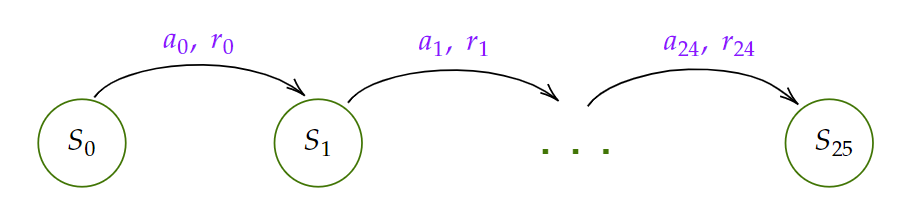
\includegraphics[width=11cm]{states_model}
		\caption{environment model}
		\label{f1equi}
	\end{figure}
	
	In \textit{action-value} methods such as Q-learning, the value of of each state or state-action pair is learned and based on these values, the policy would be determined.
	However, in \textit{Policy Gradient} methods, the policy is learnt directly without using value functions for action selection.
	
	
	Since the number of states in our model is large, we need a function approximator to to parametrize the action preferences. We use a artificial neural network for this purpose and we show the vector of connection weights in our network as $ \theta $.
	
	The actions at each state are chosen using in a way that action with higher valuation is more likely to be chosen
	
	\section{Monte Carlo Policy Gradient}
	
	\section{Reinforcement with Baseline}
	
	\section{Actor-Critic method}
		
	

	
	%\bibliographystyle{ecta}
	%\bibliographystyle{acm}
	\small
	\bibliographystyle{book}
	\bibliography{bib-evol} 
	
\end{document}